% Created 2017-02-03 Fri 07:17
% Intended LaTeX compiler: pdflatex
\documentclass[11pt]{article}
\usepackage[utf8]{inputenc}
\usepackage{lmodern}
\usepackage[T1]{fontenc}
\usepackage{fixltx2e}
\usepackage{graphicx}
\usepackage{longtable}
\usepackage{float}
\usepackage{wrapfig}
\usepackage{rotating}
\usepackage[normalem]{ulem}
\usepackage{amsmath}
\usepackage{textcomp}
\usepackage{marvosym}
\usepackage{wasysym}
\usepackage{amssymb}
\usepackage{amsmath}
\usepackage[version=3]{mhchem}
\usepackage[numbers,super,sort&compress]{natbib}
\usepackage{natmove}
\usepackage{url}
\usepackage{minted}
\usepackage{underscore}
\usepackage[linktocpage,pdfstartview=FitH,colorlinks,
linkcolor=blue,anchorcolor=blue,
citecolor=blue,filecolor=blue,menucolor=blue,urlcolor=blue]{hyperref}
\usepackage{attachfile}
\usepackage{geometry}
\geometry{margin=1.0in}
\usepackage{outline}
\usepackage{amsmath}
\usepackage{graphicx}
\usepackage{epstopdf}
\usepackage{siunitx}
\usepackage{fancyhdr}
\usepackage{hyperref}
\usepackage[labelfont=bf]{caption}
\setlength{\headheight}{15.2pt}
\def\dbar{{\mathchar'26\mkern-12mu d}}
\pagestyle{fancy}
\fancyhf{}
\renewcommand{\headrulewidth}{0.5pt}
\renewcommand{\footrulewidth}{0.5pt}
\lfoot{\today}
\cfoot{\copyright\ 2017 W.\ F.\ Schneider}
\rfoot{\thepage}
\lhead{\em{Physical Chemistry for Chemical Engineers}}
\rhead{ND CHE 30324}
\setcounter{secnumdepth}{3}
\author{William F. Schneider}
\date{\today}
\title{CHE 30324 Outline}
\begin{document}

\begin{OPTIONS}
\end{OPTIONS}


\section{The Classical Foundations}
\label{sec:org145a4fa}
\subsection{Lecture 0: Introduction}
\label{sec:org43ac82b}
\begin{enumerate}
\item Burning lighter
\item Foundations of Physical Chemistry
\begin{enumerate}
\item Quantum mechanics
\item Statistical mechanics
\item Thermodynamics, kinetics, spectroscopy
\item Physical and chemical properties of matter
\end{enumerate}
\end{enumerate}

\begin{table}
\begin{center}
\caption{Key units in Physical Chemistry}
\begin{tabular}{|lrlrl|} 
  \hline
  $N_\mathrm{Av}$: & $6.02214 \times 10^{23}$& mol$^{-1}$  & & \\
  1 amu: & $1.6605\times 10^{-27}$ & kg & & \\
  $k_\mathrm{B}$: & $1.38065\times 10^{-23}$ & J~K$^{-1}$ & $8.61734\times
  10^{-5}$ & eV K$^{-1}$\\
  $R$: & 8.314472 & J K$^{-1}$ mol$^{-1}$ & $8.2057 \times 10^{-2}$ & l atm mol$^{-1}$ K$^{-1}$\\
  $\sigma_\mathrm{SB}$: & $5.6704\times 10^{-8}$ & J s$^{-1}$ m$^{-2}$ K$^{-4}$ & & \\
  $c$: & $2.99792458\times 10^8$ & m s$^{-1}$ & & \\
  $h$: & $6.62607\times 10^{-34}$ & J s & $4.13566\times 10^{-15}$ & eV s
  \\
  $\hbar$: & $1.05457\times 10^{-34}$ & J s & $6.58212\times 10^{-16}$&  eV s \\
  $hc$: & 1239.8 & eV nm  & & \\
  $e$: & $1.60218\times 10^{-19}$ &  C & & \\
  $m_e:$ & $9.10938215\times 10^{-31}$ & kg &1:  0.5109989 & MeV c$^{-2}$  \\
  $\epsilon_0$: & $8.85419 \times 10^{-12}$ & C$^2$ J$^{-1}$ m$^{-1}$ & $5.52635\times
  10^{-3}$ & $e^2$ \AA$^{-1}$ eV$^{-1}$ \\
  $e^2/4\pi\epsilon_0$: & $2.30708 \times 10^{-28}$&  J m & 14.39964 & eV \AA\\
  $a_0$: & $0.529177 \times 10^{-10}$ & m & 0.529177 & \AA\\
  $E_\mathrm{H} $: & 1 & Ha & 27.212 & eV \\
  \hline
\end{tabular}
\end{center}
\end{table}
\subsection{Lecture 1: Basic statistics}
\label{sec:org9b3d598}
\begin{enumerate}
\item Discrete probability distributions---Coin flip
\begin{enumerate}
\item Example of Bernoulli trial, \(2^n\) possible outcomes from \(n\) flips
\item Number of ways to get \(i\) heads in \(n\) flips, \(_nC_i=n!/i!(n-i)!\)
\item Probability of \(i\) heads \(P_i \propto\ _nC_i\)
\item \emph{Normalized} probability, \(\tilde P_i = P_i/\sum_i P_i =\ _nC_i/2^n\)
\item Expectation value \(\langle i \rangle = \sum_i i \tilde P_i\)
\end{enumerate}

\item Continuous distributions---temperature
\begin{enumerate}
\item Probability density \(P(x)\) has units \(1/x\)
\item Normalized \(\tilde P(x) = P(x)/\int P(x) dx\)
\item (Unitless) probability \(a < x < b = \int_a^b \tilde P(x) dx\)
\item Expectation value \(\langle f(x) \rangle = \int f(x) \tilde P(x) dx\)
\item Mean \(= \langle x \rangle\)
\item Mean squared \(= \langle x^2 \rangle\)
\item Variance \(\sigma^2=\langle x^2 \rangle - \langle x \rangle^2\)
\item Standard deviation \(\Delta x = \sigma\)
\end{enumerate}

\item Boltzmann distribution
\begin{enumerate}
\item \(P(E) \propto e^{-E/k_BT}\), in some sense the definition of temperature
\item Energy and its units
\item Absolute temperature and its units
\item \(k_BT\) as an energy scale, \SI{0.026}{eV} at \SI{298}{K}

\item Gravity example
\begin{enumerate}
\item \(E(h)=mgh\), linear, continuous energy spectrum
\item molecule vs car in a gravitational field (Table \ref{carvelectron})
\item Barometric law for gases, \(P=P_0e^{-mgh/k_BT}\)
\end{enumerate}
\item Kinetic energy in 1-D example
\begin{enumerate}
\item \(KE = \frac{1}{2}m v_x^2\)
\item \(P_{1D}(v_x) = \left ( \frac{m}{2\pi k_B T} \right )^{1/2}\exp\left
          (-\frac{m|v_x|^2}{2 k_BT} \right )\)
\item Gaussian distribution, mean \(\mu\), variance \(\sigma^2\)
\[G(x)=\frac{1}{\sigma\sqrt{2\pi}} \exp\left (
          -\frac{(x-\mu)^2}{2\sigma^2} \right )\]
\item By inspection, \(\mu=\langle v_x \rangle=0\), \(\sigma^2=\langle v_x^2\rangle =k_BT/m\)
\item Molecule vs car again
\end{enumerate}
\item Equipartition -- energy freely exchanged between all degrees of freedom
\end{enumerate}
\end{enumerate}

\begin{table}[htbp]
\caption{Car vs gas molecule at the earth's surface \label{carvelectron}}
\centering
\begin{tabular}{lll}
\hline
 & car & gas molecule\\
\hline
\emph{m} & \SI{1000}{kg} & \SI{1e-26}{kg}\\
\emph{h} & \SI{1}{m} & \SI{1}{m}\\
\emph{mgh} & \SI{9800}{J} & \SI{9.8e-26}{J}\\
 & \SI{6.1e22}{eV} & \SI{6.1e-7}{eV}\\
\emph{T} & \SI{298}{K} & \SI{298}{K}\\
\(k_BT\) & \SI{0.026}{eV} & \SI{0.026}{eV}\\
\(mgh/k_BT\) & \SI{2.4e24}{} & \SI{2.3e-5}{}\\
\(P(\SI{1}{m})/P(0)\) & \(e^{-2.4\times 10^{-24}}\) & 0.99998\\
\(\langle h \rangle\) & \SI{0}{m} & \SI{42}{km}\\
\(\langle v_x \rangle^{1/2}\) & \SI{2e-12}{m/s} & \SI{640}{m/s}\\
\hline
\end{tabular}
\end{table}

\begin{table}\small
\begin{center}
\caption{Energy conversions and correspondences}
\begin{tabular}{|l|ccccc|}
\hline 
 & J & eV &  Hartree & kJ mol$^{-1}$ & cm$^{-1}$\\
\hline
1 J = & 1 & $6.2415\times 10^{18}$ & $2.2937\times 10^{17}$ &  $6.0221 \times
10^{20}$  & $5.0340 \times 10^{22} $\\ 
1 eV = & $1.6022 \times 10^{-19} $ & 1 & 0.036748 & 96.485 & 8065.5 \\
1 Ha = & $4.3598\times 10^{-18}$ & 27.212 & 1 & 2625.6 & 219474.6 \\
1 kJ mol$^{-1}$ = & $1.6605\times 10^{-21}$ & 0.010364 & $ 3.8087\times 10^{-4}$ & 1 & 83.5935 \\
1 cm$^{-1}$ = &$ 1.986410^{-23}$ & $1.23984\times 10^{-4}$ & $4.55623\times
10^{-6}$& 0.011963 & 1 \\
\hline 
\end{tabular}
\end{center}
\end{table}


\begin{minted}[frame=lines,fontsize=\scriptsize,linenos]{python}
import numpy as np
import matplotlib.pyplot as plt

R0 = 8.31441  # J/mol K
mass = 28. /1000 # kg/mol N2

def Boltzmann(E,T):
    return np.exp(-E/(R0*T))/(R0*T)

def MB1D(v,T):
    return np.sqrt(mass/(2*np.pi*R0*T))*np.exp(-(mass*v*v)/(2*R0*T))

def MB(c,T):
    K = 0.5 * mass * c *c
    degeneracy = 4 * np.pi * c * c
    normalization = (mass/(2*np.pi*R0*T))**1.5
    return normalization*degeneracy*Boltzmann(K,T)

energy = np.linspace(0,3000,1500)
velocity = np.linspace(-1000,1000,1000)
speed = np.linspace(0,1500,1000)

plt.figure()
for Temperature in [100,300,1000]:
   Probability = Boltzmann(energy,Temperature)
   plt.plot(Probability,energy,label='{0} K'.format(Temperature))

legend = plt.legend()

plt.ylabel('Energy (J/mol)')
plt.xlabel('Probability (mol/J)')
# plt.title('Boltzmann distribution at various temperatures')
plt.savefig('./Images/Boltzmann.png')

plt.figure()
for Temperature in [100,200,300,400,500]:
    Probability = MB1D(velocity,Temperature)
    plt.plot(velocity,Probability,label='{} K'.format(Temperature))

legend=plt.legend()
plt.xlabel('Velocity (m/s)')
plt.ylabel('Probability (1/(m/s))')
# plt.title('Boltzmann distribution at various temperatures')
plt.savefig('./Images/MB1D.png')

plt.figure()
for Temperature in [100,200,300,400,500]:
    Probability = MB(speed,Temperature)
    plt.plot(speed,Probability,label='{} K'.format(Temperature))

legend=plt.legend()
plt.xlabel('Speed (m/s)')
plt.ylabel('Probability (1/(m/s))')
# plt.title('Boltzmann distribution at various temperatures')
plt.savefig('./Images/MB.png')
\end{minted}

\begin{figure}[htbp]
\centering
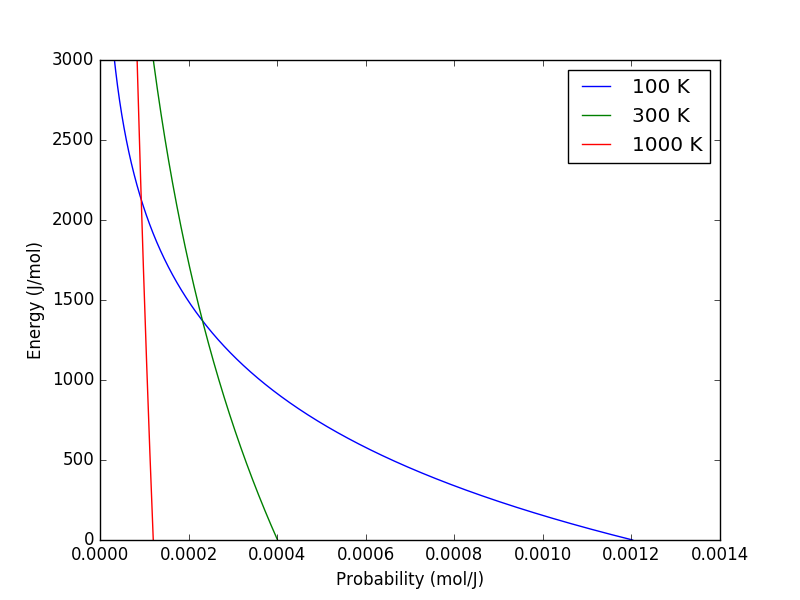
\includegraphics[width=0.5\textwidth]{./Images/Boltzmann.png}
\caption{Boltzmann distribution at various temperatures}
\end{figure}


\begin{figure}[htbp]
\centering
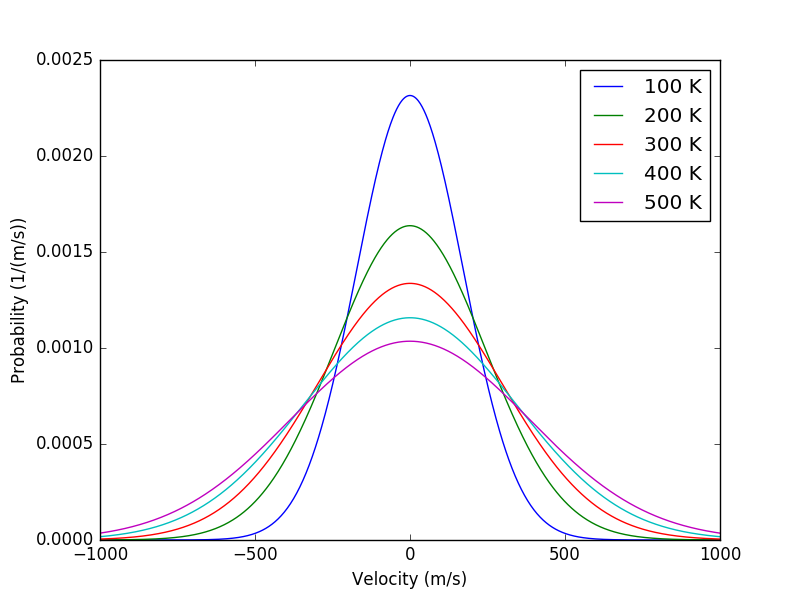
\includegraphics[width=0.5\textwidth]{./Images/MB1D.png}
\caption{One-dimensional (Gaussian) velocities of N\(_2\) gas}
\end{figure}

\begin{figure}[htbp]
\centering
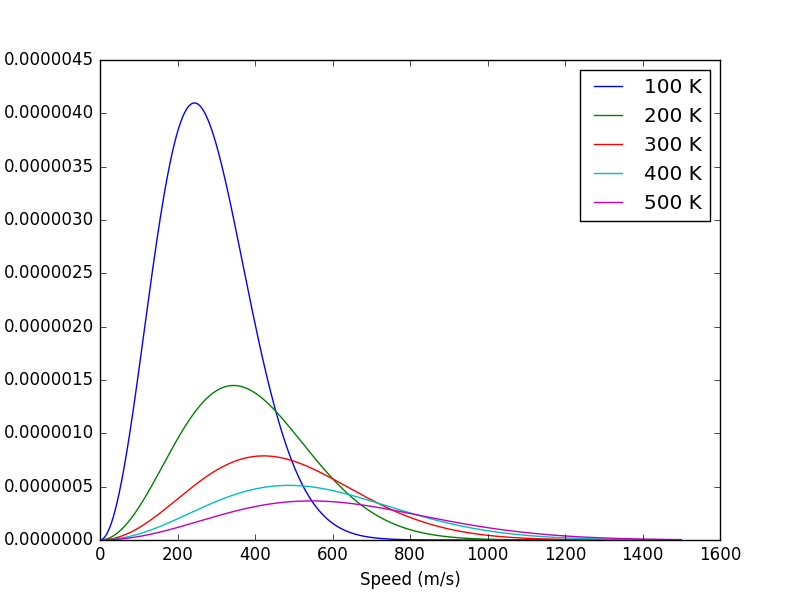
\includegraphics[width=0.5\textwidth]{./Images/MB.png}
\caption{Maxwell-Boltzmann speed distribution of N\(_2\) gas}
\end{figure}

\subsection{Lecture 2: Kinetic theory of gases}
\label{sec:org5e2c1f2}
\begin{enumerate}
\item Postulates
\begin{enumerate}
\item Gas is composed of molecules in constant random, thermal motion
\item Molecules only interact by perfectly elastic collisions
\item Volume of molecules is \(<<\) total volume
\end{enumerate}
\item Maxwell-Boltzmann distribution of molecular speeds
\begin{enumerate}
\item Speed \(v=\sqrt{v_x^2+v_y^2+v_z^2}\)
\item \(P_{MB}(v) dv = P_{1D}(v_x) P_{1D}(v_y) P_{1D}(v_z) * \text{degeneracy}(v) dv\)
\item mean speeds \(\propto \sqrt{T}\)
\item mean energy \(U=\frac{3}{2} RT\) and heat capacity \(C_v=\frac{3}{2} R\)
\end{enumerate}
\item Flux and pressure
\begin{enumerate}
\item Velocity flux \(j(v_x) dv_x= v_x \frac{N}{V}P(v_x)dv_x\), molecules /area /time /\(v_x\)
\item Wall collisions, \(J_w\), total collisions /area /time
\item Momentum exchange, pressure, ideal gas law
\end{enumerate}
\item Collisions and mean free path
\begin{enumerate}
\item Collision cross section \(\sigma=\pi d^2\), size of molecule
\item Molecular collisions, \(z\) per molecule and \(z_{\mathrm{AA}}\) per volume
\item Mean free path, \(\lambda\), mean distance between collisions
\end{enumerate}
\end{enumerate}

\begin{figure}[htbp]
\centering
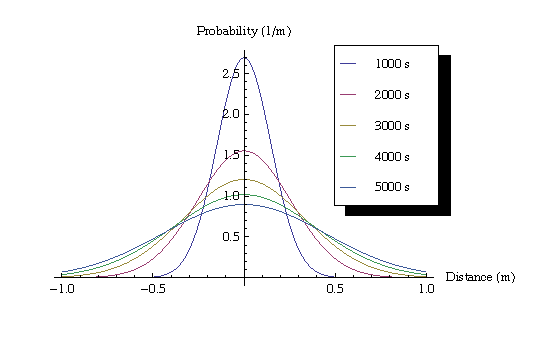
\includegraphics[width=0.6\textwidth]{./Images/Diffusion.pdf}
\caption{Diffusional spreading, \(\sqrt{\langle x^2 \rangle} = \sqrt{2 D t}\)}
\end{figure}

\begin{table} 
\begin{center}
    \caption{Kinetic theory of gases key equations}
    \begin{tabular}{|lr|}
     \hline
 & \\
Boltzmann distribution & $\displaystyle P(E) = g(E) e^{-E/k_BT}$ \\ \ \ \ \ ($g(E)$: degeneracy of
$E$) & \\ 
Maxwell-Boltzmann distribution & $ \displaystyle
P_{\rm MB}(v) = 4\pi v^2 \left( \frac{m}{2\pi k_B T}\right)^{3/2}\exp\left(-\frac{m
    v^2}{2k_B T}\right) $ \\  & \\
Mean and RMS speeds & 

$\displaystyle \langle v \rangle = \left( \frac{8 k_B T}{\pi m} \right)^{1/2} \ \ \ \ \langle v^2
\rangle^{1/2} = \left( \frac{3 k_B T}{m} \right)^{1/2} $ \\  & \\

Pressure & $
\displaystyle \langle P \rangle = \frac{\Delta p}{\Delta t} = m \frac{N}{V}\frac{1}{3}\langle v^2
\rangle = \frac{N k_B T}{V}=\frac{n R T}{V} $ \\ & \\ 

Wall collision frequency &
$ \displaystyle  J_W = \frac{1}{4}\frac{N}{V}\langle v \rangle=\frac{P}{\left( 2 \pi m k_B
    T\right)^{1/2}} $ \\ & \\

Molecular collision frequency &
$ \displaystyle  z=\sqrt{2} \sigma \langle v \rangle\frac{N}{V} = \frac{4\sigma P}{\left( \pi m k_B T
  \right)^{1/2}} $ \\ & \\

Total collisions &
$ \displaystyle z_{AA} = \frac{1}{2} \frac{N}{V} z$ \\ & \\

Mean free path &
$\displaystyle \lambda = \frac{ \langle v \rangle}{z} = \frac{V}{\sqrt{2} \sigma N} $
\\ & \\

Graham's effusion law & $\displaystyle \frac{dN}{dt}=\text{Area}\cdot  J_w \propto 1/m^{1/2} $
\\ & \\
Effusion from a vessel & $\displaystyle P=P_0 e^{-t/\tau}, \tau = \frac{V}{A}\left
  (\frac{2\pi m}{k_B T}\right )^{1/2} $ \\ & \\ 

Self-diffusion constant &
$\displaystyle D_{11} = \frac{1}{3}\langle v \rangle \lambda $ \\ & \\

Diffusion rate &
$\displaystyle \langle x^2 \rangle^{1/2} = \sqrt{2 D t} $\ \ \ \  $\langle r^2 \rangle^{1/2} = \sqrt{6
D t}$ \\ & \\

Einstein-Smoluchowski equation & $\displaystyle D_{11}= \frac{\delta^2}{2\tau}$ \\ & \\

Stokes-Einstein equation for liquids & $\displaystyle D_{11}=\frac{k_BT}{4\pi\eta r}$\ \ \
``Slip'' boundary \\
 & \\
 & $\displaystyle D_\mathrm{Brownian}=\frac{k_BT}{6\pi\eta r}$\ \ \ ``Stick'' boundary \\
\hline
    \end{tabular}
\end{center}
 \end{table}

\subsection{Lecture 3: Transport}
\label{sec:org2d08b05}
\begin{enumerate}
\item Effusion and Graham's law, \(\text{effusion rate}\propto MW^{-1/2}\)
\item Fick's first law: net flux proportional to concentration gradient
\begin{enumerate}
\item \(j_x = -D \frac{d c}{d x}\)
\item Self-diffusion constant, \(D=\frac{1}{3}\lambda \langle v \rangle\)
\end{enumerate}
\item Knudsen diffusion, \(D=\frac{1}{3}l \langle v \rangle\)
\item Fick's second law: time evolution of concentration gradient
\begin{enumerate}
\item Continuity with no advection: \(\frac{\partial c}{\partial t}
          = -\nabla\cdot \vec{j} + \text{gen}\)
\item One-dimension: \(\frac{d c}{d t} = D \frac{d^2 c}{dx^2}\)
\item Diffusion has Gaussian probability distribution: \(c(x,t)/c_0 = [2 \sqrt{\pi D
          t}]^{-1} \exp(-x^2/4Dt)\)
\end{enumerate}

\item Seeing is believing---Brownian motion
\begin{enumerate}
\item Seemingly random motion of large particles (``dust'') due to ``kicks'' from invisible molecules
\item Einstein receives Nobel Prize for showing:
\begin{enumerate}
\item Motion follows same Gaussian diffusion behavior
\item From steady-state arguments in a field, diffusion constant is ratio of Boltzmann energy, \(k_B T\), to mobility
\item Mobility inversely related to viscosity
\end{enumerate}
\item Stokes-Einstein equation
\item Allows measurement of Avogadro's number, final proof of kinetic theory
\item Similar model for diffusion of liquid molecules, slip boundary
\end{enumerate}

\item Random walk model of diffusion
\begin{enumerate}
\item Binomial distribution
\item Large \(N\) and Stirling approximation
\item Einstein-Smoluchowski relation
\end{enumerate}
\end{enumerate}

\section{Quantum Mechanics: Blurred Lines Between Particles and Waves}
\label{sec:org4538734}
\subsection{Lecture 4: Duality and demise of classical physics}
\label{sec:orgff88d31}
\subsubsection{Properties of waves}
\label{sec:org752c79d}
\begin{enumerate}
\item traveling waves, \(\psi(x,t)=A \sin(kx-\omega t)\), \(k=2\pi/\lambda\), \(\omega=2\pi\nu\)
\item standing waves, \(\psi(x,t) = A \sin(kx) \cos(\omega t)\)
\item interference, diffraction
\item energy proportional to amplitude squared
\item Expected energy of a classical oscillator, \(\langle \epsilon \rangle _\nu = k_B T\) for all \(\nu\)
\end{enumerate}

\subsubsection{Blackbody radiation}
\label{sec:org29c64b9}
\begin{enumerate}
\item Hohlraum spectrum (like the sun) empirically observed to obey:
\begin{enumerate}
\item Stefan-Boltzmann law, total irradiance
\item Wien's displacement law
\end{enumerate}
\item Rayleigh-Jeans predicts spectrum using classical physics
\begin{enumerate}
\item standing waves + classical oscillators \(\rightarrow\) ultraviolet catastrophe
\end{enumerate}
\item Planck model
\begin{enumerate}
\item Energy spectrum of oscillators are \emph{quantized}, \(\epsilon_\nu=nh\nu\)
\item Expected energy of a quantized oscillator, \(\langle \epsilon \rangle_\nu = h\nu/\left (
          e^{h\nu/k_BT}-1 \right )\)
\item Correctly reproduces Stefan-Boltzmann and Wien Laws!
\end{enumerate}
\end{enumerate}
\subsubsection{Heat capacities of solids}
\label{sec:orgfa0852f}
\begin{enumerate}
\item Law of DuLong and Pettite, \(C_v = 3R\), fails at low \(T\)
\item Einstein model
\begin{enumerate}
\item Atomic vibrations are \emph{quantized}, \(\epsilon_n=nh\nu\)
\item Heat capacity goes to zero at low \(T\)
\end{enumerate}
\end{enumerate}
\subsubsection{Photoelectric effect}
\label{sec:orgabc9476}
\begin{enumerate}
\item Stopping potential and work function, \(E_\text{kinetic}=h\nu -W\)
\item Kinetic energy varies with light frequency, number of electrons varies with light intensity
\end{enumerate}
\subsubsection{Compton effect}
\label{sec:orgcd09631}
\begin{enumerate}
\item light scattering of electrons changes \(\lambda\)
\item Photon properties, \(\epsilon = h\nu, p=h/\lambda\)
\end{enumerate}
\subsubsection{Wave-particle duality}
\label{sec:orgb0efc9e}

\begin{minted}[frame=lines,fontsize=\scriptsize,linenos]{python}
import numpy as np
import matplotlib.pyplot as plt

hc = 1239.8      # eV nm
c = 2.9979e8 * 1.e9   # nm/s
k = 8.61734e-5   # eV /K
hck = hc/k       # nm K

def Irrad(wl,T):
      return (8. * np.pi * hc * c * wl**-5) / (np.exp(hck/(wl*T))-1)
def PlanckEnergy(wl,T):
      return (hc/wl) / (np.exp(hck/(wl*T))-1)

plt.figure()
wl=np.linspace(100,5000,1000)
for T in [1000.,2000.,3000.,4000.,5000.]:
    Intensity = Irrad(wl,T)
    plt.plot(wl,Intensity,label='{} K'.format(T))

legend=plt.legend()
plt.xlabel('Wavelength (nm)')
plt.ylabel('Irradiance (eV/nm$^3$/s)')
# plt.title('Boltzmann distribution at various temperatures')
plt.savefig('./Images/BlackBody.png')

plt.figure()
color=['red','orange','green','blue','violet']
wl=np.linspace(100,20000,1000)
for T in [1000.,2000.,3000.,4000.,5000.]:
    Energy = PlanckEnergy(wl,T)
    plt.plot(wl,Energy,label='{} K'.format(T),color=color[0])
    kT = k*T
    plt.plot([100,max(wl)],[kT,kT],ls='--',color=color.pop(0))

legend=plt.legend()
plt.xlabel('Wavelength (nm)')
plt.ylabel('Energy (eV)')
# plt.title('Boltzmann distribution at various temperatures')
plt.savefig('./Images/Planck.png')
\end{minted}

\begin{figure}[htbp]
\centering
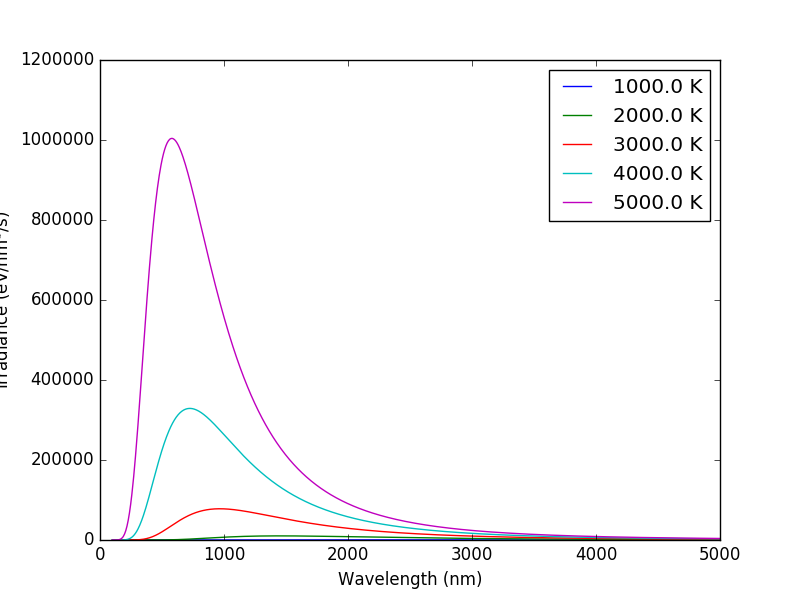
\includegraphics[width=0.5\textwidth]{./Images/BlackBody.png}
\caption{Blackbody irradiance}
\end{figure}
\begin{figure}[htbp]
\centering
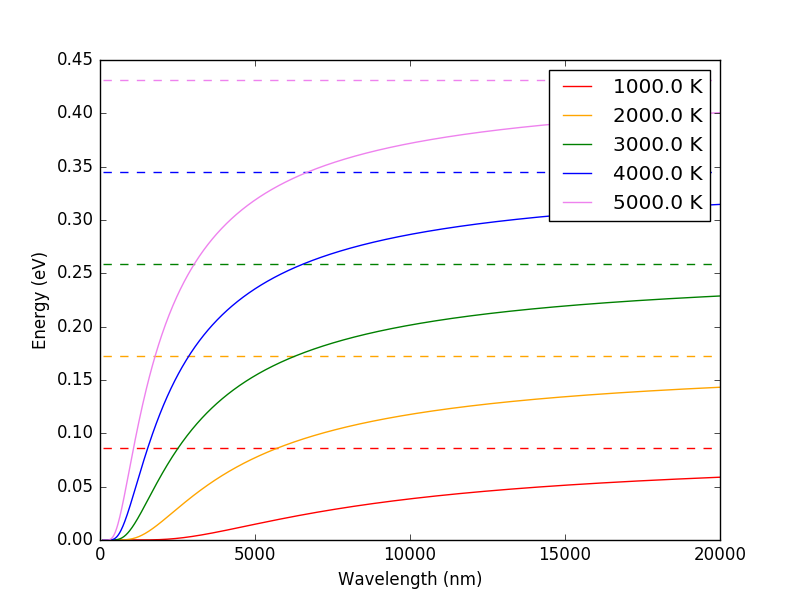
\includegraphics[width=0.5\textwidth]{./Images/Planck.png}
\caption{Average energy of a Planck quantized oscillator}
\end{figure}

\begin{table} 
\begin{center}
    \caption{The new physics}
    \begin{tabular}{|lr|}
     \hline
 & \\
Stefan-Boltzmann Law & $\displaystyle  \int I(\lambda,T)d\lambda = \sigma_\mathrm{SB} T^4$
\\ & \\
Wien's Law & $\displaystyle \lambda_\mathrm{max}T=2897768$ nm K \\
 & \\
Rayleigh-Jeans eq& $\displaystyle I(\lambda,T) = \frac{8\pi}{\lambda^4} k_B T c $ \\ 
& \\
Blackbody irradiance & $\displaystyle I(\lambda, T) =
\frac{8\pi}{\lambda^5}\frac{hc^2}{e^{hc/\lambda k_B T}-1}$ \\ 
& \\
Einstein crystal & $\displaystyle C_v=3R \left(\frac{h\nu}{k_BT}\right )^2\frac{e^{h\nu/k_BT}}{\left
            ( e^{h\nu/k_BT}-1 \right )^2}$ \\
& \\
Photon energy & $\displaystyle \epsilon=h\nu $ \\
& \\
Rydberg equation & $\displaystyle \nu = R_H c\left (1/n^2
        -1/k^2 \right)$ \\
& \\
Bohr equations & $\displaystyle l_n=n \hbar$ \\
$\displaystyle n=1,2, \ldots $ & $\displaystyle r_n = n^2 \left ( \frac{4 \pi
    \epsilon_0 \hbar^2}{e^2 m_e} \right ) = n^2 a_0$ \\
 & $\displaystyle E_n =-\frac{m_e e^4}{8\epsilon_0^2
   h^2}\frac{1}{n^2}=-\frac{E_H}{2}\frac{1}{n^2}$ \\ 
 & $\displaystyle p_n =\frac{e^2}{4\pi\epsilon_0}\frac{m_e}{\hbar}\frac{1}{n} =
p_0 \frac{1}{n} $ \\
& \\
de Broglie equation & $\displaystyle \lambda=h/p $ \\
\hline
\end{tabular}
\end{center}
\end{table}

\section{Statistical Mechanics: The Bridge from the Tiny to the Many}
\label{sec:org440c166}
\end{document}